\documentclass[14pt]{extarticle}

\usepackage{amsmath,mathtools,amsfonts,amsthm,amssymb,hyperref,wasysym,xcolor}
\usepackage{parskip,geometry,latexsym,bookmark,mathtools,float,cancel,tcolorbox}

\newtheorem{defn}{Definition}
\newtheorem{thm}{Theorem}
\newtheorem{claim}{Claim}
\newtheorem{lemma}{Lemma}

\newcommand{\dps}{\displaystyle}
\newcommand{\fbl}{\underline{\hspace{1cm}}\,\,}
\newcommand{\R}{\mathbb{R}}
\newcommand{\Z}{\mathbb{Z}}
\newcommand{\Q}{\mathbb{Q}}
\newcommand{\from}{\leftarrow}
\newcommand{\true}{{\bf t}}
\newcommand{\false}{{\bf c}}
\newcommand{\bic}{\leftrightarrow}
\newcommand{\base}[1]{{\color{cyan}#1}}
\newcommand{\da}{\downarrow}
\newcommand{\fa}{\forall}
\newcommand{\te}{\exists}

\hypersetup{colorlinks,allcolors=blue,linktoc=all}
\geometry{a4paper}
\geometry{margin=0.5in}

\title{Chapter 3 Solutions, Susanna Epp Discrete Math 5th Edition}

\author{https://github.com/spamegg1}

\begin{document}
\maketitle
\tableofcontents

\section{Exercise Set 3.1}

\subsection{Exercise 1}
A menagerie consists of seven brown dogs, two black dogs, six gray cats, ten black cats, five blue birds, six yellow birds, and one black bird. Determine which of the following statements are true and which are false.

\subsubsection{(a)}
There is an animal in the menagerie that is red.

\begin{proof}

\end{proof}

\subsubsection{(b)}
Every animal in the menagerie is a bird or a mammal.
\begin{proof}

\end{proof}

\subsubsection{(c)}
Every animal in the menagerie is brown or gray or black.
\begin{proof}

\end{proof}

\subsubsection{(d)}
There is an animal in the menagerie that is neither a cat nor a dog.
\begin{proof}

\end{proof}

\subsubsection{(e)}
No animal in the menagerie is blue.

\begin{proof}

\end{proof}

\subsubsection{(f)}
There are in the menagerie a dog, a cat, and a bird that all have the same color.
\begin{proof}

\end{proof}

\subsection{Exercise 2}
Indicate which of the following statements are true and which are false. Justify your answers as best as you can.

\subsubsection{(a)}

\begin{proof}
Every integer is a real number.
\end{proof}

\subsubsection{(b)}
0 is a positive real number.
\begin{proof}

\end{proof}

\subsubsection{(c)}
For every real number r, 2r is a negative real number.
\begin{proof}

\end{proof}

\subsubsection{(d)}
Every real number is an integer.
\begin{proof}

\end{proof}

\subsection{Exercise 3}
Let $R(m, n)$ be the predicate “If $m$ is a factor of $n^2$ then $m$ is a factor of $n$,” with domain for both $m$ and $n$ being $\Z$ the set of integers.

\subsubsection{(a)}
Explain why $R(m, n)$ is false if $m = 25$ and $n = 10$.
\begin{proof}

\end{proof}

\subsubsection{(b)}
Give values different from those in part (a) for which $R(m, n)$ is false.

\begin{proof}

\end{proof}

\subsubsection{(c)}
Explain why $R(m, n)$ is true if $m = 5$ and $n = 10$.

\begin{proof}

\end{proof}

\subsubsection{(d)}
Give values different from those in part (c) for which $R(m, n)$ is true.

\begin{proof}

\end{proof}

\subsection{Exercise 4}
Let $Q(x, y)$ be the predicate “If $x < y$ then $x^2 < y^2$” with domain for both $x$ and $y$ being $\R$ the set of real numbers.

\subsubsection{(a)}
Explain why $Q(x, y)$ is false if $x = -2$ and $y = 1$.

\begin{proof}

\end{proof}

\subsubsection{(b)}
Give values different from those in part (a) for which $Q(x, y)$ is false.

\begin{proof}

\end{proof}

\subsubsection{(c)}
Explain why $Q(x, y)$ is true if $x = 3$ and $y = 8$.

\begin{proof}

\end{proof}

\subsubsection{(d)}
Give values different from those in part (c) for which $Q(x, y)$ is true.

\begin{proof}

\end{proof}

\subsection{Exercise 5}
Find the truth set of each predicate.

\subsubsection{(a)}
Predicate: $6/d$ is an integer, domain: $\Z$

\begin{proof}

\end{proof}

\subsubsection{(b)}
Predicate: $6/d$ is an integer, domain: $\Z^+$

\begin{proof}

\end{proof}

\subsubsection{(c)}
Predicate: $1 \leq x_2 \leq 4$, domain: $\R$

\begin{proof}

\end{proof}

\subsubsection{(d)}
Predicate: $1 \leq x_2 \leq 4$, domain: $\Z$

\begin{proof}

\end{proof}

\subsection{Exercise 6}
Let $B(x)$ be “$-10 < x < 10$.” Find the truth set of $B(x)$ for each of the following domains.

\subsubsection{(a)}
$\Z$

\begin{proof}

\end{proof}

\subsubsection{(b)}
$\Z^+$
 
\begin{proof}

\end{proof}

\subsubsection{(c)}
The set of all even integers

\begin{proof}

\end{proof}

\subsection{Exercise 7}
Let $S$ be the set of all strings of length 3 consisting of $a$’s, $b$’s, and $c$’s. List all the strings in $S$ that satisfy the following conditions:

1. Every string in $S$ begins with $b$.

2. No string in $S$ has more than one $c$.

\begin{proof}

\end{proof}

\subsection{Exercise 8}
Let $T$ be the set of all strings of length 3 consisting of 0’s and 1’s. List all the strings in $T$ that satisfy the following conditions:

1. For every string $s$ in $T$, the second character of $s$ is 1 or the first two characters of $s$ are the same.

2. No string in $T$ has all three characters the same.

\begin{proof}

\end{proof}

{\bf \color{cyan} Find counterexamples to show that the statements in 9–12 are false.}

\subsection{Exercise 9}
$\fa x \in \R, x \geq 1/x$

\begin{proof}

\end{proof}

\subsection{Exercise 10}
$\fa a \in \Z, (a-1)/a$ is not an integer.

\begin{proof}

\end{proof}

\subsection{Exercise 11}
$\fa$ positive integers $m$ and $n$, $m \cdot n \geq m + n$.

\begin{proof}

\end{proof}

\subsection{Exercise 12}
$\fa$ real numbers $x, y$, $\sqrt{x + y} = \sqrt{x} + \sqrt{y}$.
\begin{proof}

\end{proof}

\subsection{Exercise 13}
Consider the following statement: $\fa$ basketball player $x$, $x$ is tall.

Which of the following are equivalent ways of expressing this statement?

\subsubsection{(a)}
Every basketball player is tall.

\begin{proof}

\end{proof}

\subsubsection{(b)}
Among all the basketball players, some are tall.

\begin{proof}

\end{proof}

\subsubsection{(c)}
Some of all the tall people are basketball players.

\begin{proof}

\end{proof}

\subsubsection{(d)}
Anyone who is tall is a basketball player.

\begin{proof}

\end{proof}

\subsubsection{(e)}
All people who are basketball players are tall.

\begin{proof}

\end{proof}

\subsubsection{(f)}
Anyone who is a basketball player is a tall person.

\begin{proof}

\end{proof}

\subsection{Exercise 14}
Consider the following statement: $\te x \in \R$ such that $x^2 = 2$.

Which of the following are equivalent ways of expressing this statement?

\subsubsection{(a)}
The square of each real number is 2.

\begin{proof}

\end{proof}

\subsubsection{(b)}
Some real numbers have square 2.

\begin{proof}

\end{proof}

\subsubsection{(c)}
The number $x$ has square 2, for some real number $x$.

\begin{proof}

\end{proof}

\subsubsection{(d)}
If $x$ is a real number, then $x^2 = 2$.

\begin{proof}

\end{proof}

\subsubsection{(e)}
Some real number has square 2.

\begin{proof}

\end{proof}

\subsubsection{(f)}
There is at least one real number whose square is 2.

\begin{proof}

\end{proof}

\subsection{Exercise 15}
Rewrite the following statements informally in at least two different ways without using variables or quantifiers.

\subsubsection{(a)}
$\fa$ rectangle $x$, $x$ is a quadrilateral.

\begin{proof}

\end{proof}

\subsubsection{(b)}
$\te$ a set $A$ such that $A$ has 16 subsets.

\begin{proof}

\end{proof}

\subsection{Exercise 16}
Rewrite each of the following statements in the
form “$\fa \fbl x, \fbl$.”

\subsubsection{(a)}
All dinosaurs are extinct.

\begin{proof}

\end{proof}

\subsubsection{(b)}
Every real number is positive, negative, or zero.

\begin{proof}

\end{proof}

\subsubsection{(c)}
No irrational numbers are integers.

\begin{proof}

\end{proof}

\subsubsection{(d)}
No logicians are lazy.

\begin{proof}

\end{proof}

\subsubsection{(e)}
The number 2,147,581,953 is not equal to the square of any integer.

\begin{proof}

\end{proof}

\subsubsection{(f)}
The number 21 is not equal to the square of any real number.

\begin{proof}

\end{proof}

\subsection{Exercise 17}
Rewrite each of the following in the form “$\te \fbl x$ such that \fbl.”

\subsubsection{(a)}
Some exercises have answers.

\begin{proof}

\end{proof}

\subsubsection{(b)}
Some real numbers are rational.

\begin{proof}

\end{proof}

\subsection{Exercise 18}
Let $D$ be the set of all students at your school, and let $M(s)$ be “$s$ is a math major,” let $C(s)$ be “$s$ is a computer science student,” and let $E(s)$ be “$s$ is an engineering student.” Express each of the following statements using quantifiers, variables, and the predicates $M(s), C(s)$, and $E(s)$.

\subsubsection{(a)}
There is an engineering student who is a math major.

\begin{proof}

\end{proof}

\subsubsection{(b)}
Every computer science student is an engineering student.

\begin{proof}

\end{proof}

\subsubsection{(c)}
No computer science students are engineering students.

\begin{proof}

\end{proof}

\subsubsection{(d)}
Some computer science students are also math majors.

\begin{proof}

\end{proof}

\subsubsection{(e)}
Some computer science students are engineering students and some are not.

\begin{proof}

\end{proof}

\subsection{Exercise 19}
Consider the following statement: $\fa$ integer $n$, if $n^2$ is even then $n$ is even.

Which of the following are equivalent ways of expressing this statement?

\subsubsection{(a)}
All integers have even squares and are even.
\begin{proof}

\end{proof}

\subsubsection{(b)}
Given any integer whose square is even, that integer is itself even.

\begin{proof}

\end{proof}

\subsubsection{(c)}
For all integers, there are some whose square is even.

\begin{proof}

\end{proof}

\subsubsection{(d)}
Any integer with an even square is even.

\begin{proof}

\end{proof}

\subsubsection{(e)}
If the square of an integer is even, then that integer is even.

\begin{proof}

\end{proof}

\subsubsection{(f)}
All even integers have even squares.

\begin{proof}

\end{proof}

\subsection{Exercise 20}
Rewrite the following statement informally in at least two different ways without using variables or the symbol $\fa$ or the words “for all.”

$\fa$ real numbers $x$, if $x$ is positive then the square root of $x$ is positive.

\begin{proof}

\end{proof}

\subsection{Exercise 21}
Rewrite the following statements so that the quantifier trails the rest of the sentence.

\subsubsection{(a)}
For any graph $G$, the total degree of $G$ is even.

\begin{proof}

\end{proof}

\subsubsection{(b)}
For any isosceles triangle $T$, the base angles of $T$ are equal.

\begin{proof}

\end{proof}

\subsubsection{(c)}
There exists a prime number $p$ such that $p$ is even.

\begin{proof}

\end{proof}

\subsubsection{(d)}
There exists a continuous function $f$ such that $f$ is not differentiable.

\begin{proof}

\end{proof}

\subsection{Exercise 22}
Rewrite each of the following statements in the
form “$\fa \fbl x$, if \fbl then \fbl.”

\subsubsection{(a)}
All Java programs have at least 5 lines.

\begin{proof}

\end{proof}

\subsubsection{(b)}
Any valid argument with true premises has a true conclusion.

\begin{proof}

\end{proof}

\subsection{Exercise 23}
Rewrite each of the following statements in the two forms “$\fa x$, if \fbl then \fbl” and “$\fa x$, \fbl” (without an if-then).

\subsubsection{(a)}
All equilateral triangles are isosceles.

\begin{proof}

\end{proof}

\subsubsection{(b)}
Every computer science student needs to take data structures.

\begin{proof}

\end{proof}

\subsection{Exercise 24}
Rewrite the following statements in the two forms “$\te \fbl x$ such that \fbl” and “$\te x$ such that \fbl and \fbl.”

\subsubsection{(a)}

\begin{proof}
Some hatters are mad.

\end{proof}

\subsubsection{(b)}
Some questions are easy.

\begin{proof}

\end{proof}

\subsection{Exercise 25}
The statement “The square of any rational number is rational” can be rewritten formally as “For all rational numbers $x$, $x^2$ is rational” or as “For all $x$, if $x$ is rational then $x^2$ is rational.” Rewrite each of the following statements in the two forms “$\fa \fbl x$, \fbl” and “$\fa x$, if \fbl, then \fbl” or in the two forms “$\fa \fbl x$ and $y$, ”\fbl and “$\fa x$ and $y$, if \fbl, then \fbl.”

\subsubsection{(a)}
The reciprocal of any nonzero fraction is a fraction.

\begin{proof}

\end{proof}

\subsubsection{(b)}
The derivative of any polynomial function is a polynomial function.
\begin{proof}

\end{proof}

\subsubsection{(c)}
The sum of the angles of any triangle is 180°.

\begin{proof}

\end{proof}

\subsubsection{(d)}
The negative of any irrational number is irrational.

\begin{proof}

\end{proof}

\subsubsection{(e)}
The sum of any two even integers is even.

\begin{proof}

\end{proof}

\subsubsection{(f)}
The product of any two fractions is a fraction.

\begin{proof}

\end{proof}

\subsection{Exercise 26}
Consider the statement “All integers are rational numbers but some rational numbers are not integers.”

\subsubsection{(a)}
Write this statement in the form “$\fa x$, if \fbl then \fbl, but $\te \fbl x$ such that \fbl.”

\begin{proof}

\end{proof}

\subsubsection{(b)}
Let Ratl($x$) be “$x$ is a rational number” and Int($x$) be “$x$ is an integer.” Write the given statement formally using only the symbols Ratl($x$), Int($x$), $\fa, \te, \wedge, \vee, \sim,$ and $\to$.

\begin{proof}

\end{proof}

\subsection{Exercise 27}
Refer to the picture of Tarski’s world given in Example 3.1.13. Let Above($x, y$) mean that $x$ is above $y$ (but possibly in a different column). Determine the truth or falsity of each of the following statements. Give reasons for your answers.

\subsubsection{(a)}
$\fa u$, Circle($u$) $\to$ Gray($u$).

\begin{proof}

\end{proof}

\subsubsection{(b)}
$\fa u$, Gray($u$) $\to$ Circle($u$).

\begin{proof}

\end{proof}

\subsubsection{(c)}
$\te y$ such that Square($y$) $\wedge$ Above($y, d$).

\begin{proof}

\end{proof}

\subsubsection{(d)}
$\te z$ such that Triangle($z$) $\wedge$ Above($f, z$).
\begin{proof}

\end{proof}

{\bf \color{cyan} In $28-30$, rewrite each statement without using quantifiers or variables. Indicate which are true and which are false, and justify your answers as best as you can.}

\subsection{Exercise 28}
Let the domain of $x$ be the set $D$ of objects discussed in mathematics courses, and let Real($x$) be “$x$ is a real number,” Pos($x$) be “$x$ is a positive real number,” Neg($x$) be “$x$ is a negative real number,” and Int($x$) be “$x$ is an integer.”

\subsubsection{(a)}
Pos(0)

\begin{proof}

\end{proof}

\subsubsection{(b)}
$\fa x$, Real($x$) $\wedge$ Neg($x$) $\to$ Pos($-x$)

\begin{proof}

\end{proof}

\subsubsection{(c)}
$\fa x$, Int($x$) $\to$ Real$(x)$

\begin{proof}

\end{proof}

\subsubsection{(d)}
$\te x$ such that, Real($x$) $\wedge$ $\sim$ Int($x$) 

\begin{proof}

\end{proof}

\subsection{Exercise 29}
Let the domain of $x$ be the set of geometric figures in the plane, and let Square($x$) be “$x$ is a square” and Rect($x$) be “$x$ is a rectangle.”

\subsubsection{(a)}
$\te x$ such that Rect($x$) $\wedge$ Square($x$)

\begin{proof}

\end{proof}

\subsubsection{(b)}
$\te x$ such that Rect($x$) $\wedge \sim$ Square($x$)

\begin{proof}

\end{proof}

\subsubsection{(c)}
$\fa x$, Square($x$) $\to$ Rect($x$)

\begin{proof}

\end{proof}

\subsection{Exercise 30}
Let the domain of $x$ be $\Z$, the set of integers, and let Odd($x$) be “$x$ is odd,” Prime($x$) be “$x$ is prime,” and Square($x$) be “$x$ is a perfect square.” (An integer $n$ is said to be a perfect square if, and only if, it equals the square of some integer. For example, 25 is a perfect square because $25 = 5^2$.)

\subsubsection{(a)}
$\te x$ such that Prime($x$) $\wedge\sim$Odd($x$)

\begin{proof}

\end{proof}

\subsubsection{(b)}
$\fa x$, Prime($x$) $\to$ $\sim$Square($x$)

\begin{proof}

\end{proof}

\subsubsection{(c)}
$\te x$ such that Odd($x$) $\wedge$ Square($x$)

\begin{proof}

\end{proof}

\subsection{Exercise 31}
In any mathematics or computer science text other than this book, find an example of a statement that is universal but is implicitly quantified. Copy the statement as it appears and rewrite it making the quantification explicit. Give a complete citation for your example, including title, author, publisher,
year, and page number.

\begin{proof}

\end{proof}

\subsection{Exercise 32}
Let $\R$ be the domain of the predicate variable $x$. Which of the following are true and which are false? Give counter examples for the statements that are false.

\subsubsection{(a)}
$x > 2 \implies x > 1$

\begin{proof}

\end{proof}

\subsubsection{(b)}
$x > 2 \implies x^2 > 4$

\begin{proof}

\end{proof}

\subsubsection{(c)}
$x^2 > 4 \implies x > 2$

\begin{proof}

\end{proof}

\subsubsection{(d)}
$x^2 > 4 \iff |x| > 2$

\begin{proof}

\end{proof}

\subsection{Exercise 33}
Let $\R$ be the domain of the predicate variables $a, b, c$, and $d$. Which of the following are true and which are false? Give counterexamples for the statements that are false.

\subsubsection{(a)}
$a > 0$ and $b > 0 \implies ab > 0$

\begin{proof}

\end{proof}

\subsubsection{(b)}
$a < 0$ and $b < 0 \implies ab < 0$

\begin{proof}

\end{proof}

\subsubsection{(c)}
$ab = 0 \implies a = 0$ or $b = 0$

\begin{proof}

\end{proof}

\subsubsection{(d)}
$a < b$ and $c < d \implies ac < bd$

\begin{proof}

\end{proof}

\section{Exercise Set 3.2}

\subsection{Exercise 1}
Which of the following is a negation for “All discrete mathematics students are athletic”? More than one answer may be correct.

\subsubsection{(a)}
There is a discrete mathematics student who is nonathletic.

\begin{proof}

\end{proof}

\subsubsection{(b)}
All discrete mathematics students are nonathletic.

\begin{proof}

\end{proof}

\subsubsection{(c)}
There is an athletic person who is not a discrete mathematics student.

\begin{proof}

\end{proof}

\subsubsection{(d)}
No discrete mathematics students are athletic.

\begin{proof}

\end{proof}

\subsubsection{(e)}
Some discrete mathematics students are nonathletic.

\begin{proof}

\end{proof}

\subsubsection{(f)}
No athletic people are discrete mathematics students.

\begin{proof}

\end{proof}

\subsection{Exercise 2}
Which of the following is a negation for “All dogs
are loyal”? More than one answer may be correct.

\subsubsection{(a)}
All dogs are disloyal.

\begin{proof}

\end{proof}

\subsubsection{(b)}
No dogs are loyal.

\begin{proof}

\end{proof}

\subsubsection{(c)}
Some dogs are disloyal.

\begin{proof}

\end{proof}

\subsubsection{(d)}
Some dogs are loyal.

\begin{proof}

\end{proof}

\subsubsection{(e)}
There is a disloyal animal that is not a dog.

\begin{proof}

\end{proof}

\subsubsection{(f)}
There is a dog that is disloyal.

\begin{proof}

\end{proof}

\subsubsection{(g)}
No animals that are not dogs are loyal.

\begin{proof}

\end{proof}

\subsubsection{(h)}
Some animals that are not dogs are loyal.

\begin{proof}

\end{proof}

\subsection{Exercise 3}
Write a formal negation for each of the following statements.

\subsubsection{(a)}
$\fa$ string $s$, $s$ has at least one character.

\begin{proof}

\end{proof}

\subsubsection{(b)}
$\fa$ computer $c$, $c$ has a CPU.

\begin{proof}

\end{proof}

\subsubsection{(c)}
$\te$ a movie $m$ such that $m$ is over 6 hours long.

\begin{proof}

\end{proof}

\subsubsection{(d)}
$\te$ a band $b$ such that $b$ has won at least 10 Grammy awards.

\begin{proof}

\end{proof}

\subsection{Exercise 4}
Write an informal negation for each of the following statements. Be careful to avoid negations that are ambiguous.

\subsubsection{(a)}
All dogs are friendly.

\begin{proof}

\end{proof}

\subsubsection{(b)}
All graphs are connected.

\begin{proof}

\end{proof}

\subsubsection{(c)}
Some suspicions were substantiated.

\begin{proof}

\end{proof}

\subsubsection{(d)}
Some estimates are accurate.

\begin{proof}

\end{proof}

\subsection{Exercise 5}
Write a negation for each of the following statements.

\subsubsection{(a)}
Every valid argument has a true conclusion.

\begin{proof}

\end{proof}

\subsubsection{(b)}
All real numbers are positive, negative, or zero.

\begin{proof}

\end{proof}

{\bf \color{cyan}Write a negation for each statement in 6 and 7.}

\subsection{Exercise 6}

\subsubsection{(a)}
Sets $A$ and $B$ do not have any points in common.

\begin{proof}

\end{proof}

\subsubsection{(b)}
Towns $P$ and $Q$ are not connected by any road on the map.

\begin{proof}

\end{proof}

\subsection{Exercise 7}

\subsubsection{(a)}
This vertex is not connected to any other vertex in the graph.

\begin{proof}

\end{proof}

\subsubsection{(b)}
This number is not related to any even number.

\begin{proof}

\end{proof}

\subsection{Exercise 8}
Consider the statement “There are no simple solutions to life’s problems.” Write an informal negation for the statement, and then write the statement formally using quantifiers and variables.

\begin{proof}

\end{proof}

{\bf \color{cyan}Write a negation for each statement in 9 and 10.}

\subsection{Exercise 9}
$\fa$ real number $x$, if $x > 3$ then $x^2 > 9$.

\begin{proof}

\end{proof}

\subsection{Exercise 10}
$\fa$ computer program $P$, if $P$ compiles without error messages, then $P$ is correct.

\begin{proof}

\end{proof}

{\bf \color{cyan} In each of $11-14$ determine whether the proposed negation is correct. If it is not, write a correct negation.}

\subsection{Exercise 11}
Statement: The sum of any two irrational numbers is irrational.

Proposed negation: The sum of any two irrational numbers is rational.

\begin{proof}

\end{proof}

\subsection{Exercise 12}
Statement: The product of any irrational number and any rational number is irrational.

Proposed negation: The product of any irrational number and any rational number is rational.

\begin{proof}

\end{proof}

\subsection{Exercise 13}
Statement: For every integer $n$, if $n^2$ is even then $n$ is even.

Proposed negation: For every integer $n$, if $n^2$ is even then $n$ is not even.

\begin{proof}

\end{proof}

\subsection{Exercise 14}
Statement: For all real numbers $x_1$ and $x_2$, if $x_1^2 = x_2^2$ then $x_1 = x_2$.

Proposed negation: For all real numbers $x_1$ and $x_2$, if $x_1^2 = x_2^2$ then $x1 \neq x2$.

\begin{proof}

\end{proof}

\subsection{Exercise 15}
Let D 5 {248,214,28, 0, 1, 3, 16, 23, 26, 32, 36}.
Determine which of the following statements are
true and which are false. Provide counterexamples
for the statements that are false.

\subsubsection{(a)}
$\fa x \in D$, if $x$ is odd then $x > 0$.

\begin{proof}

\end{proof}

\subsubsection{(b)}
$\fa x \in D$, if $x$ is less than 0 then $x$ is even.

\begin{proof}

\end{proof}

\subsubsection{(c)}
$\fa x \in D$, if $x$ is even then $x \leq 0$.

\begin{proof}

\end{proof}

\subsubsection{(d)}
$\fa x \in D$, if the ones digit of $x$ is 2, then the tens digit is 3 or 4.

\begin{proof}

\end{proof}

\subsubsection{(e)}
$\fa x \in D$, if the ones digit of $x$ is 6, then the tens digit is 1 or 2.

\begin{proof}

\end{proof}

{\bf \color{cyan} In $16-23$, write a negation for each statement.}

\subsection{Exercise 16}
$\fa$ real number $x$, if $x^2 \geq 1$ then $x > 0$.

\begin{proof}

\end{proof}

\subsection{Exercise 17}
$\fa$ integer $d$, if $6 / d$ is an integer then $d = 3$.

\begin{proof}

\end{proof}

\subsection{Exercise 18}
$\fa x \in \R$, if $x(x + 1) > 0$ then $x > 0$ or $x < -1$.

\begin{proof}

\end{proof}

\subsection{Exercise 19}
$\fa n \in \Z$, if $n$ is prime then $n$ is odd or $n = 2$.

\begin{proof}

\end{proof}

\subsection{Exercise 20}
$\fa$ integers $a, b$, and $c$, if $a - b$ is even and $b - c$ is even, then $a - c$ is even.

\begin{proof}

\end{proof}

\subsection{Exercise 21}
$\fa$ integer $n$, if $n$ is divisible by 6, then $n$ is divisible by 2 and $n$ is divisible by 3.

\begin{proof}

\end{proof}

\subsection{Exercise 22}
If the square of an integer is odd, then the integer is odd.

\begin{proof}

\end{proof}

\subsection{Exercise 23}
If a function is differentiable then it is continuous.

\begin{proof}

\end{proof}

\subsection{Exercise 24}
Rewrite the statements in each pair in if-then form
and indicate the logical relationship between them.

\subsubsection{(a)}
All the children in Tom’s family are female. 

All the females in Tom’s family are children.

\begin{proof}

\end{proof}

\subsubsection{(b)}
All the integers that are greater than 5 and end in 1, 3, 7, or 9 are prime. 

All the integers that are greater than 5 and are prime end in 1, 3, 7, or 9.

\begin{proof}

\end{proof}

\subsection{Exercise 25}
Each of the following statements is true. In each case write the converse of the statement, and give a counterexample showing that the converse is false.

\subsubsection{(a)}
If $n$ is any prime number that is greater than 2, then $n + 1$ is even.

\begin{proof}

\end{proof}

\subsubsection{(b)}
If $m$ is any odd integer, then $2m$ is even.

\begin{proof}

\end{proof}

\subsubsection{(c)}
If two circles intersect in exactly two points, then they do not have a common center.

\begin{proof}

\end{proof}

{\bf \color{cyan} In $26-33$, for each statement in the referenced exercise write the contrapositive, converse, and inverse. Indicate as best as you can which of these statements are true and which are false. Give a counterexample for each that is false.}

\subsection{Exercise 26}
Exercise 16 

\begin{proof}

\end{proof}

\subsection{Exercise 27}
Exercise 17

\begin{proof}

\end{proof}

\subsection{Exercise 28}
Exercise 18

\begin{proof}

\end{proof}

\subsection{Exercise 29}
Exercise 19

\begin{proof}

\end{proof}

\subsection{Exercise 30}
Exercise 20

\begin{proof}

\end{proof}

\subsection{Exercise 31}
Exercise 21

\begin{proof}

\end{proof}

\subsection{Exercise 32}
Exercise 22

\begin{proof}

\end{proof}

\subsection{Exercise 33}
Exercise 23

\begin{proof}

\end{proof}

\subsection{Exercise 34}
Write the contrapositive for each of the following statements.

\subsubsection{(a)}
If $n$ is prime, then $n$ is not divisible by any prime number from 2 through $\sqrt{n}$. (Assume that $n$ is a fixed integer.)

\begin{proof}

\end{proof}

\subsubsection{(b)}
If $A$ and $B$ do not have any elements in common, then they are disjoint. (Assume that $A$ and $B$ are fixed sets.)

\begin{proof}

\end{proof}

\subsection{Exercise 35}
Give an example to show that a universal conditional statement is not logically equivalent to its inverse.

\begin{proof}

\end{proof}

\subsection{Exercise 36}
If $P(x)$ is a predicate and the domain of $x$ is the set of all real numbers, let $R$ be “$\fa x \in \Z, P(x)$,” let $S$ be “$\fa x \in \Q, P(x)$,” and let $T$ be “$\fa x \in \R, P(x)$.”

\subsubsection{(a)}
Find a definition for $P(x)$ (but do not use “$x \in \Z$”) so that $R$ is true and both $S$ and $T$ are false.

\begin{proof}

\end{proof}

\subsubsection{(b)}
Find a definition for $P(x)$ (but do not use “$x \in \Q$”) so that both $R$ and $S$ are true and $T$ is false.

\begin{proof}

\end{proof}

\subsection{Exercise 37}
Consider the following sequence of digits: 0204. A person claims that all the 1’s in the sequence are to the left of all the 0’s in the sequence. Is this true? Justify your answer. (Hint: Write the claim formally and write a formal negation for it. Is the negation true or false?)

\begin{proof}

\end{proof}

\subsection{Exercise 38}
True or false? All occurrences of the letter $u$ in {\it Discrete Mathematics} are lowercase. Justify your answer.

\begin{proof}

\end{proof}

{\bf \color{cyan} Rewrite each statement of 39–44 in if-then form.}

\subsection{Exercise 39}
Earning a grade of C2 in this course is a sufficient condition for it to count toward graduation.
\begin{proof}

\end{proof}

\subsection{Exercise 40}
Being divisible by 8 is a sufficient condition for being divisible by 4.
\begin{proof}

\end{proof}

\subsection{Exercise 41}
Being on time each day is a necessary condition for keeping this job.

\begin{proof}

\end{proof}

\subsection{Exercise 42}
Passing a comprehensive exam is a necessary condition for obtaining a master’s degree.

\begin{proof}

\end{proof}

\subsection{Exercise 43}
A number is prime only if it is greater than 1.

\begin{proof}

\end{proof}

\subsection{Exercise 44}
A polygon is square only if it has four sides.

\begin{proof}

\end{proof}

{\bf \color{cyan} Use the facts that the negation of a $\fa$ statement is a $\te$ statement and that the negation of an if-then statement is an and statement to rewrite each of the statements $45-48$ without using the word necessary or sufficient.}

\subsection{Exercise 45}
Being divisible by 8 is not a necessary condition for being divisible by 4.

\begin{proof}

\end{proof}

\subsection{Exercise 46}
Having a large income is not a necessary condition for a person to be happy.

\begin{proof}

\end{proof}

\subsection{Exercise 47}
Having a large income is not a sufficient condition for a person to be happy.

\begin{proof}

\end{proof}

\subsection{Exercise 48}
Being a polynomial is not a sufficient condition for a function to have a real root.

\begin{proof}

\end{proof}

\subsection{Exercise 49}
The computer scientists Richard Conway and David Gries once wrote:

The absence of error messages during translation of a computer program is only a necessary and not a sufficient condition for
reasonable [program] correctness.

Rewrite this statement without using the words necessary or sufficient.

\begin{proof}

\end{proof}

\subsection{Exercise 50}
A frequent-flyer club brochure states, “You may select among carriers only if they offer the same lowest fare.” Assuming that “only if” has its formal, logical meaning, does this statement guarantee that if two carriers offer the same lowest fare, the customer will be free to choose between them? Explain.

\begin{proof}

\end{proof}

\section{Exercise Set 3.3}
\subsection{Exercise 1}
Let $C$ be the set of cities in the world, let $N$ be the set of nations in the world, and let $P(c, n)$ be “$c$ is the capital city of $n$.” Determine the truth values of the following statements.

\subsubsection{(a)}
$P$(Tokyo, Japan)

\begin{proof}

\end{proof}

\subsubsection{(b)}
$P$(Athens, Egypt)

\begin{proof}

\end{proof}

\subsubsection{(c)}
$P$(Paris, France)

\begin{proof}

\end{proof}

\subsubsection{(d)}
$P$(Miami, Brazil)

\begin{proof}

\end{proof}

\subsection{Exercise 2}
Let $G(x, y)$ be “$x^2 > y$.” Indicate which of the following statements are true and which are false.

\subsubsection{(a)}
$G(2, 3)$

\begin{proof}

\end{proof}

\subsubsection{(b)}
$G(1, 1)$

\begin{proof}

\end{proof}

\subsubsection{(c)}
$G(1/2, 1/2)$

\begin{proof}

\end{proof}

\subsubsection{(d)}
$G(-2, 2)$

\begin{proof}

\end{proof}

\subsection{Exercise 3}
The following statement is true: “$\fa$ nonzero number $x$, $\te$ a real number $y$ such that $xy = 1$.” For each $x$ given below, find a $y$ to make the predicate “$xy = 1$” true.

\subsubsection{(a)}
$x = 2$

\begin{proof}

\end{proof}

\subsubsection{(b)}
$x = -1$

\begin{proof}

\end{proof}

\subsubsection{(c)}
$x = 3/4$

\begin{proof}

\end{proof}

\subsection{Exercise 4}
The following statement is true: “$\fa$ real number $x$, $\te$ an integer $n$ such that $n > x$.” For each $x$ given below, find an $n$ to make the predicate “$n > x$” true.

\subsubsection{(a)}
$x = 15.83$

\begin{proof}

\end{proof}

\subsubsection{(b)}
$x = 10^8$

\begin{proof}

\end{proof}

\subsubsection{(c)}
$x = 10^{10^{10}}$

\begin{proof}

\end{proof}

\begin{figure}[ht!]
\centering
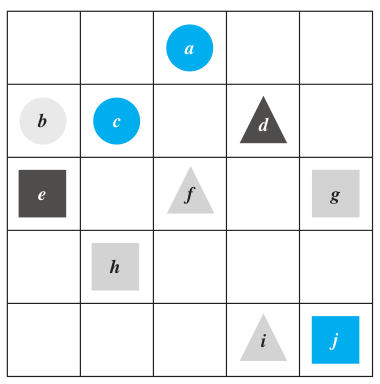
\includegraphics[scale=0.4]{../images/3.3.1.png}
\end{figure}

{\bf \color{cyan} The statements in exercises $5-8$ refer to the Tarski world given in Figure 3.3.1 (repeated above). Explain why each is true.}

\subsection{Exercise 5}
For every circle $x$ there is a square $y$ such that $x$ and $y$ have the same color.

\begin{proof}

\end{proof}

\subsection{Exercise 6}
For every square $x$ there is a circle $y$ such that $x$ and $y$ have different colors and $y$ is above $x$.

\begin{proof}

\end{proof}

\subsection{Exercise 7}
There is a triangle $x$ such that for every square $y$, $x$ is above $y$.

\begin{proof}

\end{proof}

\subsection{Exercise 8}
There is a triangle $x$ such that for every circle $y$, $y$ is above $x$.

\begin{proof}

\end{proof}

\subsection{Exercise 9}
Let $D = E = \{-2, -1, 0, 1, 2\}$. Explain why the following statements are true.

\subsubsection{(a)}
$\fa x$ in $D$, $\te y$ in $E$ such that $x + y = 0$.

\begin{proof}

\end{proof}

\subsubsection{(b)}
$\te x$ in $D$ such that $\fa y$ in $E$, $x + y = y$.

\begin{proof}

\end{proof}

\subsection{Exercise 10}
This exercise refers to Example 3.3.3. Determine whether each of the following statements is true or false.

\subsubsection{(a)}
$\fa$ student $S$, $\te$ a dessert $D$ such that $S$ chose $D$.

\begin{proof}

\end{proof}

\subsubsection{(b)}
$\fa$ student $S$, $\te$ a salad $T$ such that $S$ chose $T$.

\begin{proof}

\end{proof}

\subsubsection{(c)}
$\te$ a dessert $D$ such that $\fa$ student $S$, $S$ chose $D$.

\begin{proof}

\end{proof}

\subsubsection{(d)}
$\te$ a beverage $B$ such that $\fa$ student $D$, $D$ chose $B$.

\begin{proof}

\end{proof}

\subsubsection{(e)}
$\te$ an item $I$ such that $\fa$ student $S$, $S$ did not choose $I$.

\begin{proof}

\end{proof}

\subsubsection{(f)}
$\te$ a station $Z$ such that $\fa$ student $S$, $\te$ an item $I$ such that $S$ chose $I$ from $Z$.

\begin{proof}

\end{proof}

\subsection{Exercise 11}
Let $S$ be the set of students at your school, let $M$ be the set of movies that have ever been released, and let $V(s, m)$ be “student $s$ has seen movie $m$.” Rewrite each of the following statements without using the symbol $\fa$, the symbol $\te$, or variables.

\subsubsection{(a)}
$\te s \in S$ such that $V(s$, Casablanca).

\begin{proof}

\end{proof}

\subsubsection{(b)}
$\fa s \in S$, $V(s$, Star Wars).

\begin{proof}

\end{proof}

\subsubsection{(c)}
$\fa s \in S$, $\te m \in M$ such that $V(s, m)$.

\begin{proof}

\end{proof}

\subsubsection{(d)}
$\te m \in M$ such that $\fa s \in S$, $V(s, m)$.

\begin{proof}

\end{proof}

\subsubsection{(e)}
$\te s \in S$, $\te t \in S$, and $\te m \in M$ such that $s \neq t$ and $V(s, m) \wedge V(t, m)$.

\begin{proof}

\end{proof}

\subsubsection{(f)}
$\te s \in S$ and $\te t \in S$ such that $s \neq t$ and $\fa m \in M$, $V(s, m) \to V(t, m)$.

\begin{proof}

\end{proof}

\subsection{Exercise 12}
Let $D = E = \{-2, -1, 0, 1, 2\}$. Write negations for each of the following statements and determine which is true, the given statement or its negation.

\subsubsection{(a)}
$\fa x$ in $D$, $\te y$ in $E$ such that $x + y = 1$.

\begin{proof}

\end{proof}

\subsubsection{(b)}
$\te x$ in $D$ such that $\fa y$ in $E$, $x + y = -y$.

\begin{proof}

\end{proof}

\subsubsection{(c)}
$\fa x$ in $D$, $\te y$ in $E$ such that $xy \geq y$.

\begin{proof}

\end{proof}

\subsubsection{(d)}
$\te x$ in $D$ such that $\fa y$ in $E$, $x \leq y$.

\begin{proof}

\end{proof}

{\bf \color{cyan} In each of $13-19$, (a) rewrite the statement in English without using the symbol $\fa$ or $\te$ or variables and expressing your answer as simply as possible, and (b) write a negation for the statement.}

\subsection{Exercise 13}
$\fa$ color $C$, $\te$ an animal $A$ such that $A$ is colored $C$.

\begin{proof}

\end{proof}

\subsection{Exercise 14}
$\te$ a book $b$ such that $\fa$ person $p$, $p$ has read $b$.

\begin{proof}

\end{proof}

\subsection{Exercise 15}
$\fa$ odd integer $n$, $\te$ an integer $k$ such that $n = 2k + 1$.

\begin{proof}

\end{proof}

\subsection{Exercise 16}
$\te$ a real number $u$ such that $\fa$ real number $v$, $uv = v$.

\begin{proof}

\end{proof}

\subsection{Exercise 17}
$\fa r \in \Q$, $\te$ integers $a$ and $b$ such that $r = a/b$.

\begin{proof}

\end{proof}

\subsection{Exercise 18}
$\fa x \in \R$, $\te$ a real number $y$ such that $x + y = 0$.
\begin{proof}

\end{proof}

\subsection{Exercise 19}
$\te x \in \R$ such that for every real number $y$, $x + y = 0$.
\begin{proof}

\end{proof}

\subsection{Exercise 20}
\begin{figure}[ht!]
\centering
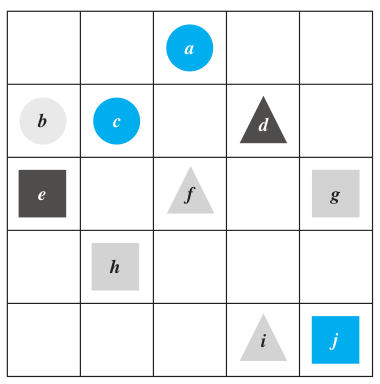
\includegraphics[scale=0.4]{../images/3.3.1.png}
\end{figure}

Recall that reversing the order of the quantifiers in a statement with two different quantifiers may change the truth value of the statement, but it does not necessarily do so. All the statements in the pairs below refer to the Tarski world of Figure 3.3.1. In each pair, the order of the quantifiers is reversed but everything else is the same. For each pair, determine whether the statements have the same or opposite truth values. Justify your answers.

\subsubsection{(a)}
(1) For every square $y$ there is a triangle $x$ such that $x$ and $y$ have different colors.

(2) There is a triangle $x$ such that for every square $y$, $x$ and $y$ have different colors.

\begin{proof}

\end{proof}

\subsubsection{(b)}
(1) For every circle $y$ there is a square $x$ such that $x$ and $y$ have the same color.

(2) There is a square $x$ such that for every circle $y$, $x$ and $y$ have the same color.

\begin{proof}

\end{proof}

\subsection{Exercise 21}
For each of the following equations, determine which of the following statements are true:

(1) For every real number $x$, there exists a real number $y$ such that the equation is true.

(2) There exists a real number $x$, such that for every real number $y$, the equation is true.

Note that it is possible for both statements to be true or for both to be false.

\subsubsection{(a)}
$2x + y = 7$

\begin{proof}

\end{proof}

\subsubsection{(b)}
$y + x = x + y$

\begin{proof}

\end{proof}

\subsubsection{(c)}
$x^2 - 2xy + y^2 = 0$

\begin{proof}

\end{proof}

\subsubsection{(d)}
$(x - 5)(y - 1) = 0$

\begin{proof}

\end{proof}

\subsubsection{(e)}
$x^2 + y^2 = -1$

\begin{proof}

\end{proof}

{\bf \color{cyan} In 22 and 23, rewrite each statement without using variables or the symbol $\fa$ or $\te$. Indicate whether the statement is true or false.}

\subsection{Exercise 22}
\subsubsection{(a)}
$\fa$ real number $x$, $\te$ a real number $y$ such that $x + y = 0$.

\begin{proof}

\end{proof}

\subsubsection{(b)}
$\te$ a real number $y$ such that $\fa$ real number $x$, $x + y = 0$.

\begin{proof}

\end{proof}

\subsection{Exercise 23}
\subsubsection{(a)}
$\fa$ nonzero real number $r$, $\te$ a real number $s$ such that $rs = 1$.

\begin{proof}

\end{proof}

\subsubsection{(b)}
$\te$ a real number $r$ such that $\fa$ nonzero real number $s$, $rs = 1$.

\begin{proof}

\end{proof}

\subsection{Exercise 24}
Use the laws for negating universal and existential statements to derive the following rules:

\subsubsection{(a)}
$\sim(\fa x \in D(\fa y \in E(P(x, y)))) \equiv \te x \in D(\te y \in E({\sim P(x, y)}))$

\begin{proof}

\end{proof}

\subsubsection{(b)}
$\sim(\te x \in D(\te y \in E(P(x, y)))) \equiv \fa x \in D(\fa y \in E({\sim P(x, y)}))$

\begin{proof}

\end{proof}

\begin{figure}[ht!]
\centering
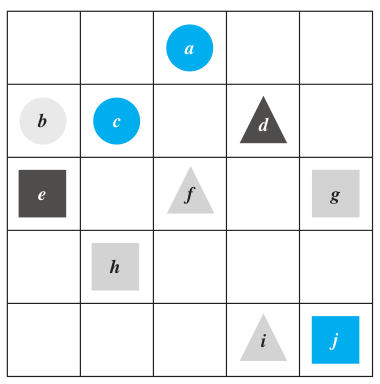
\includegraphics[scale=0.4]{../images/3.3.1.png}
\end{figure}

{\bf \color{cyan} Each statement in $25-28$ refers to the Tarski world of Figure 3.3.1 (repeated above). For each, (a) determine whether the statement is true or false and justify your answer, and (b) write a negation for the statement (referring, if you wish, to the result in exercise 24).}

\subsection{Exercise 25}
$\fa$ circle $x$ and $\fa$ square $y$, $x$ is above $y$.

\begin{proof}

\end{proof}

\subsection{Exercise 26}
$\fa$ circle $x$ and $\fa$ triangle $y$, $x$ is above $y$.

\begin{proof}

\end{proof}

\subsection{Exercise 27}
$\te$ a circle $x$ and $\te$ a square $y$ such that $x$ is above $y$ and $x$ and $y$ have different colors.

\begin{proof}

\end{proof}

\subsection{Exercise 28}
$\te$ a triangle $x$ and $\te$ a square $y$ such that $x$ is above $y$ and $x$ and $y$ have the same color.

\begin{proof}

\end{proof}

{\bf \color{cyan} For each of the statements in 29 and 30, (a) write a new statement by interchanging the symbols $\fa$ and $\te$, and (b) state which is true: the given statement, the version with interchanged quantifiers, neither, or both.}

\subsection{Exercise 29}
$\fa x \in \R, \te y \in \R$ such that $x < y$.

\begin{proof}

\end{proof}

\subsection{Exercise 30}
$\te x \in \R$ such that $\fa y \in \R^-$ (the set of negative real numbers), $x > y$.

\begin{proof}

\end{proof}

\subsection{Exercise 31}
Consider the statement “Everybody is older than somebody.” Rewrite this statement in the form “$\fa$ people $x$, $\te$ \fbl.”

\begin{proof}

\end{proof}

\subsection{Exercise 32}
Consider the statement “Somebody is older than everybody.” Rewrite this statement in the form “$\te$ a person $x$ such that $\fa$ \fbl.”

\begin{proof}

\end{proof}

{\bf \color{cyan} In $33-39$, (a) rewrite the statement formally using quantifiers and variables, and (b) write a negation for the statement.}

\subsection{Exercise 33}
Everybody loves somebody.

\begin{proof}

\end{proof}

\subsection{Exercise 34}
Somebody loves everybody.

\begin{proof}

\end{proof}

\subsection{Exercise 35}
Everybody trusts somebody.

\begin{proof}

\end{proof}

\subsection{Exercise 36}
Somebody trusts everybody.

\begin{proof}

\end{proof}

\subsection{Exercise 37}
Any even integer equals twice some integer.

\begin{proof}

\end{proof}

\subsection{Exercise 38}
Every action has an equal and opposite reaction.

\begin{proof}

\end{proof}

\subsection{Exercise 39}
There is a program that gives the correct answer to every question that is posed to it.

\begin{proof}

\end{proof}

\subsection{Exercise 40}
In informal speech most sentences of the form “There is \fbl every \fbl” are intended to be understood as meaning “$\fa$ \fbl $\te$ \fbl,” even though the existential quantifier {\it there is} comes before the universal quantifier {\it every}. Note that this interpretation applies to the following well-known sentences. Rewrite them using quantifiers and variables.

\subsubsection{(a)}
There is a sucker born every minute.

\begin{proof}

\end{proof}

\subsubsection{(b)}
There is a time for every purpose under heaven.

\begin{proof}

\end{proof}

\subsection{Exercise 41}
Indicate which of the following statements are true and which are false. Justify your answers as best you can.

\subsubsection{(a)}
$\fa x \in \Z^+ \te y \in \Z^+$ such that $x = y + 1$.

\begin{proof}

\end{proof}

\subsubsection{(b)}
$\fa x \in \Z \te y \in \Z$ such that $x = y + 1$.

\begin{proof}

\end{proof}

\subsubsection{(c)}
$\te x \in \R$ such that $\fa y \in \R$, $x = y + 1$.

\begin{proof}

\end{proof}

\subsubsection{(d)}
$\fa x \in \R^+ \te y \in \R^+$ such that $xy = 1$.

\begin{proof}

\end{proof}

\subsubsection{(e)}
$\fa x \in \R \te y \in \R$ such that $xy = 1$.

\begin{proof}

\end{proof}

\subsubsection{(f)}
$\te x \in \R$ such that $\fa y \in \R$, $x + y = y$.

\begin{proof}

\end{proof}

\subsubsection{(g)}
$\te x \in \R$ such that $\fa y \in \R$, $y < x$.

\begin{proof}

\end{proof}

\subsubsection{(h)}
$\te x \in \R^+$ such that $\fa y \in \R^+$, $x \leq y$.

\begin{proof}

\end{proof}

\subsection{Exercise 42}
Write the negation of the definition of limit of a sequence given in Example 3.3.7.

\begin{proof}

\end{proof}

\subsection{Exercise 43}
The following is the definition for $\lim_{x \to a} f(x) = L$:

For every real number $\epsilon > 0$, there exists a real number $\delta > 0$ such that for every real number $x$, if $a - \delta < x < a + \delta$ and $x \neq a$ then 
$$
L - \epsilon < f(x) < L + \epsilon
$$

Write what it means for $\lim_{x \to a} f(x) \neq L$. In other words, write the negation of the definition.

\begin{proof}

\end{proof}

\subsection{Exercise 44}
The notation $\te$! stands for the words “there exists a unique.” Thus, for instance, “$\te$! $x$ such that $x$ is prime and $x$ is even” means that there is one and only one even prime number. Which of the following statements are true and which are false? Explain.

\subsubsection{(a)}
$\te$! real number $x$ such that $\fa$ real number $y$, $xy = y$.

\begin{proof}

\end{proof}

\subsubsection{(b)}
$\te$! integer $x$ such that $1/x$ is an integer.

\begin{proof}

\end{proof}

\subsubsection{(c)}
$\fa$ real number $x$, $\te$! real number $y$ such that $x + y = 0$.

\begin{proof}

\end{proof}

\subsection{Exercise 45}
Suppose that $P(x)$ is a predicate and $D$ is the domain of $x$. Rewrite the statement “$\te$! $x \in D$ such that $P(x)$” without using the symbol $\te$!. (See exercise 44 for the meaning of $\te$!.)

\begin{proof}

\end{proof}

\begin{figure}[ht!]
\centering
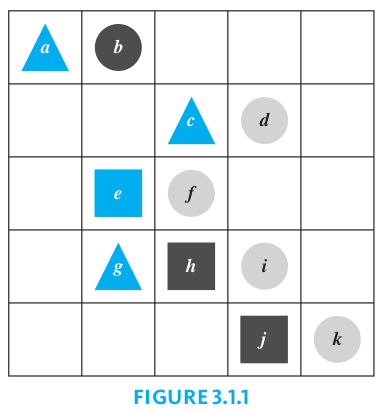
\includegraphics[scale=0.4]{../images/3.1.1.png}
\end{figure}

{\bf \color{cyan} In $46-54$, refer to the Tarski world given in Figure 3.1.1, which is shown again here for reference. the domains of all variables consist of all the objects in the Tarski world. For each statement, (a) indicate whether the statement is true or false and justify your answer, (b) write the given statement using the formal logical notation illustrated in example 3.3.10, and (c) write a negation for the given statement using the formal logical notation of example 3.3.10.}

\subsection{Exercise 46}
There is a triangle $x$ such that for every square $y$, $x$ is above $y$.

\begin{proof}

\end{proof}

\subsection{Exercise 47}
There is a triangle $x$ such that for every circle $y$, $x$ is above $y$.

\begin{proof}

\end{proof}

\subsection{Exercise 48}
For every circle $x$, there is a square $y$ such that $y$ is to the right of $x$.

\begin{proof}

\end{proof}

\subsection{Exercise 49}
For every object $x$, if $x$ is a circle then there is a square $y$ such that $y$ has the same color as $x$.

\begin{proof}

\end{proof}

\subsection{Exercise 50}
For every object $x$, if $x$ is a triangle then there is a square $y$ such that $y$ is below $x$.

\begin{proof}

\end{proof}

\subsection{Exercise 51}
There is a square $x$ such that for every triangle $y$, if $y$ is above $x$ then $y$ has the same color as $x$.

\begin{proof}

\end{proof}

\subsection{Exercise 52}
For every circle $x$ and for every triangle $y$, $x$ is to the right of $y$.

\begin{proof}

\end{proof}

\subsection{Exercise 53}
There is a circle $x$ and there is a square $y$ such that $x$ and $y$ have the same color.

\begin{proof}

\end{proof}

\subsection{Exercise 54}
There is a circle $x$ and there is a triangle $y$ such that $x$ has the same color as $y$.

\begin{proof}

\end{proof}

{\bf \color{cyan} Let $P(x)$ and $Q(x)$ be predicates and suppose $D$ is the domain of $x$. In $55-58$, for the statement forms in each pair, determine whether (a) they have the same truth value for every choice of $P(x), Q(x)$, and $D$, or (b) there is a choice of $P(x), Q(x)$, and $D$ for which they have opposite truth values.}

\subsection{Exercise 55}
$\fa x \in D, (P(x) \wedge Q(x))$, and $(\fa x \in D, P(x)) \wedge (\fa x \in D, Q(x))$

\begin{proof}

\end{proof}

\subsection{Exercise 56}
$\te x \in D, (P(x) \wedge Q(x))$, and $(\te x \in D, P(x)) \wedge (\te x \in D, Q(x))$

\begin{proof}

\end{proof}

\subsection{Exercise 57}
$\fa x \in D, (P(x) \vee Q(x))$, and $(\fa x \in D, P(x)) \vee (\fa x \in D, Q(x))$

\begin{proof}

\end{proof}

\subsection{Exercise 58}
$\te x \in D, (P(x) \vee Q(x))$, and $(\te x \in D, P(x)) \vee (\te x \in D, Q(x))$

\begin{proof}

\end{proof}

{\bf \color{cyan} In $59-61$, find the answers Prolog would give if the following questions were added to the program given in example 3.3.11.}

\subsection{Exercise 59}

\subsubsection{(a)}
?isabove$(b_1, w_1)$

\begin{proof}

\end{proof}

\subsubsection{(b)}
?color($X$, white)

\begin{proof}

\end{proof}

\subsubsection{(c)}
?isabove$(X, b_3)$

\begin{proof}

\end{proof}

\subsection{Exercise 60}

\subsubsection{(a)}
?isabove$(w_1, g)$

\begin{proof}

\end{proof}

\subsubsection{(b)}
?color$(w_2$, blue)

\begin{proof}

\end{proof}

\subsubsection{(c)}
?isabove$(X, b_1)$

\begin{proof}

\end{proof}

\subsection{Exercise 61}

\subsubsection{(a)}
?isabove$(w_2, b_3)$

\begin{proof}

\end{proof}

\subsubsection{(b)}
?color($X$, gray)

\begin{proof}

\end{proof}

\subsubsection{(c)}
?isabove$(g, X)$

\begin{proof}

\end{proof}

\section{Exercise Set 3.4}

\subsection{Exercise 1}

\subsubsection{(a)}

\begin{proof}

\end{proof}

\subsubsection{(b)}

\begin{proof}

\end{proof}

\subsubsection{(c)}

\begin{proof}

\end{proof}

\subsubsection{(d)}

\begin{proof}

\end{proof}

\subsubsection{(e)}

\begin{proof}

\end{proof}

\subsection{Exercise 2}

\begin{proof}

\end{proof}

\subsection{Exercise 3}

\begin{proof}

\end{proof}

\subsection{Exercise 4}

\begin{proof}

\end{proof}

\subsection{Exercise 5}

\begin{proof}

\end{proof}

\subsection{Exercise 6}

\begin{proof}

\end{proof}

\subsection{Exercise 7}

\begin{proof}

\end{proof}

\subsection{Exercise 8}

\begin{proof}

\end{proof}

\subsection{Exercise 9}

\begin{proof}

\end{proof}

\subsection{Exercise 10}

\begin{proof}

\end{proof}

\subsection{Exercise 11}

\begin{proof}

\end{proof}

\subsection{Exercise 12}

\begin{proof}

\end{proof}

\subsection{Exercise 13}

\begin{proof}

\end{proof}

\subsection{Exercise 14}

\begin{proof}

\end{proof}

\subsection{Exercise 15}

\begin{proof}

\end{proof}

\subsection{Exercise 16}

\begin{proof}

\end{proof}

\subsection{Exercise 17}

\begin{proof}

\end{proof}

\subsection{Exercise 18}

\begin{proof}

\end{proof}

\subsection{Exercise 19}

\subsubsection{(a)}

\begin{proof}

\end{proof}

\subsubsection{(b)}

\begin{proof}

\end{proof}

\subsubsection{(c)}

\begin{proof}

\end{proof}

\subsubsection{(d)}

\begin{proof}

\end{proof}

\subsection{Exercise 20}

\subsubsection{(a)}

\begin{proof}

\end{proof}

\subsubsection{(b)}

\begin{proof}

\end{proof}

\subsection{Exercise 21}

\begin{proof}

\end{proof}

\subsection{Exercise 22}

\begin{proof}

\end{proof}

\subsection{Exercise 23}

\begin{proof}

\end{proof}

\subsection{Exercise 24}

\begin{proof}

\end{proof}

\subsection{Exercise 25}

\begin{proof}

\end{proof}

\subsection{Exercise 26}

\begin{proof}

\end{proof}

\subsection{Exercise 27}

\begin{proof}

\end{proof}

\subsection{Exercise 28}

\begin{proof}

\end{proof}

\subsection{Exercise 29}

\begin{proof}

\end{proof}

\subsection{Exercise 30}

\begin{proof}

\end{proof}

\subsection{Exercise 31}

\begin{proof}

\end{proof}

\subsection{Exercise 32}

\begin{proof}

\end{proof}

\subsection{Exercise 33}

\begin{proof}

\end{proof}

\subsection{Exercise 34}

\begin{proof}

\end{proof}

\subsection{Exercise 35}

\begin{proof}

\end{proof}

\subsection{Exercise 36}

\begin{proof}

\end{proof}

\end{document}
